%! TeX Program = LuaLaTeX
% spell-checker: enable

\documentclass{article}

\newdimen\Lmargin
\newdimen\Rmargin
\Lmargin=1in \advance\Lmargin by\hoffset \advance\Lmargin by\oddsidemargin
\Rmargin=\paperwidth \advance\Rmargin by-\Lmargin \advance\Rmargin by-\textwidth
\ifdim\Lmargin>\Rmargin \Rmargin=\Lmargin \fi
\def\Scentering{\leftskip=0pt plus 1fil minus \Rmargin
                \rightskip=\leftskip}

\usepackage{graphicx,microtype,amsmath,multirow}

\begin{document}

\title{Relationship Between the Acceleration and Mass}
\author{Jing Huang}
\date{\today}
\maketitle

\begin{abstract}
  The acceleration and the mass are two fundamental physics quantities that I found interesting.
  Every single object has mass as its intrinsic property, while every moving object has acceleration.
  When I was in middle school, our physics teacher told us that the mass will affect how far the car can move with the given constant acceleration.
  It's not hard for me to imagine but really hard for me to explain why.
  Then in high school I learned about kinematics.
  I began to realize maybe it's because there are some sorts of relationship between the acceleration of the object and the object's mass since this explains everything.

  The Newton's second law enabled me to make a link from the theory we learned in class and my question.
  Therefore I attempted to fond out the relationship between the acceleration and the mass.
\end{abstract}

\section{Theoretical Information}

\subsection{Basis Theory}

The Newton's second law of motion is been used.
The law:
\begin{quote}
  When a body is acted upon by a net force, the body's acceleration multiplied by its mass is equal to the net force.
\end{quote}
can be represented in equation as:
\[
  F = ma.
\]

In the experiment I designed, the force is kept unchanged to make life easier, and thus we can deduct:
\[
  a = \frac{F}{m}.
\]
This leads to our consequence that the acceleration and the mass is inversely proportional.

\subsection{Theoretical Deduction}

The equipments are placed in figure~\ref{fig:equip}.
\begin{figure}
  \centering
  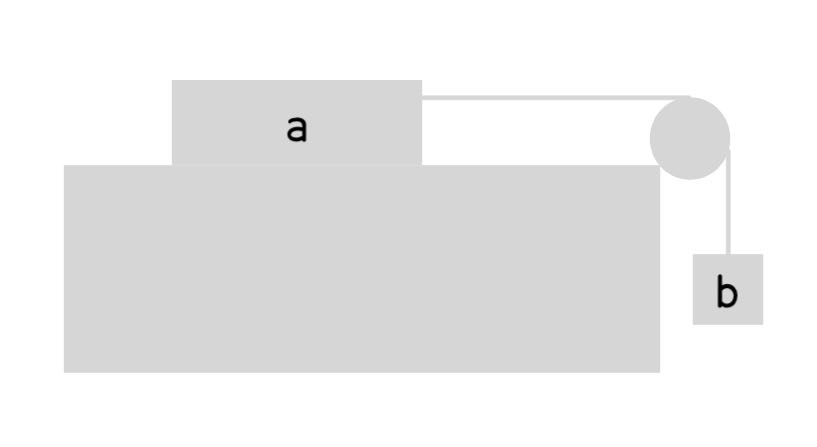
\includegraphics[width=.78\hsize]{equip.jpeg}
  \caption{The equipment used in the experiment}
  \label{fig:equip}
\end{figure}

Since the two parts of the equipment is connected by a string and their acceleration is the same,
we can see them as one object, and there is two forces acting on it:
\begin{enumerate}
  \item The weight of part b of the object $W_b$;
  \item The friction exerted on part a of the object $f_d$.
\end{enumerate}
Therefore, we can take these variables and apply them using Newton's second law:
\[
  a = \frac{F_n}{m}.
\]

To simplify, we also assume that the surface is perfectly smooth and has no friction force $f_d = 0 \text{N}$.
So the net force of this object is:
\[
  F_n = W + f_d = W.
\]

So now the relationship we found between the acceleration and the mass is:
\[
  a = \frac{W}{m} = \frac{m_b \cdot g}{m_a + m_b}.
\]
The acceleration is equivalent to the quotient of the product of the object b's mass and gravitational acceleration and the total mass of the object.

\section{Variables}

\subsection{Independent Variables}

We say a variable is independent means that the variable that changes and affects the value of the variable which we are going to evaluate.
Here, it is the mass of the entire object, or more specifically, the mass of the object a which is represented as $m_a$.
In this experiment, this variable will be changed by adding heavy objects which mass is a constant on the object a.
Its mass is measured with a electronic scale.

\subsection{Dependent Variables}

The dependent variable changes according to the independent variable, and in our case is the acceleration $a$.
We use a sensor to plot its speed-time graph, and calculate the acceleration by applying $a = \frac{v}{t}$ to it.

\subsection{Controlled Variables}

\begin{itemize}
  \item The mass of the object b is controlled to ensure the initial force is the same every time.
  \item The mass of the heavy objects to be added on the car is a constant.
  \item The coefficient friction of the surface $\mu$ is 0 for simplicity.
\end{itemize}

\section{Methodology}

\subsection{Experimental Apparatus}

\begin{enumerate}
  \item A track that has very little friction and is long enough for the car to move.
  \item A car which is tied to a heavy object.
  \item A sensor which collects the time-displacement data.
  \item A scale which can measure the mass of the car and the heavy object.
  \item A heavy object which is heavy enough  to ensure the robustness of the data measured.
  \item Some heavy object to add extra weight to the car.
\end{enumerate}

\subsection{Experimental Procedure}

\begin{enumerate}
  \item Set up all the apparatus mentioned as shown in figure~\ref{fig:setup}.
  \item At first do not place any heavy objects on the car.
  \item Connect the sensor to the computer with Vernier Logger Pro software installed and opened.
  \item Place the car at a suitable position on the track so that there is a relatively long distance for the car to move before it stops.
  \item Release the car and click the collect button on the PC.
  \item Measure for three times and add two heavy object to the car.
  \item Iterate from step 4.
\end{enumerate}

\subsection{Experimental Set-up}

The set-up diagram of the experiment is shown in figure~\ref{fig:setup}

\begin{figure}[htb]
  \centering
  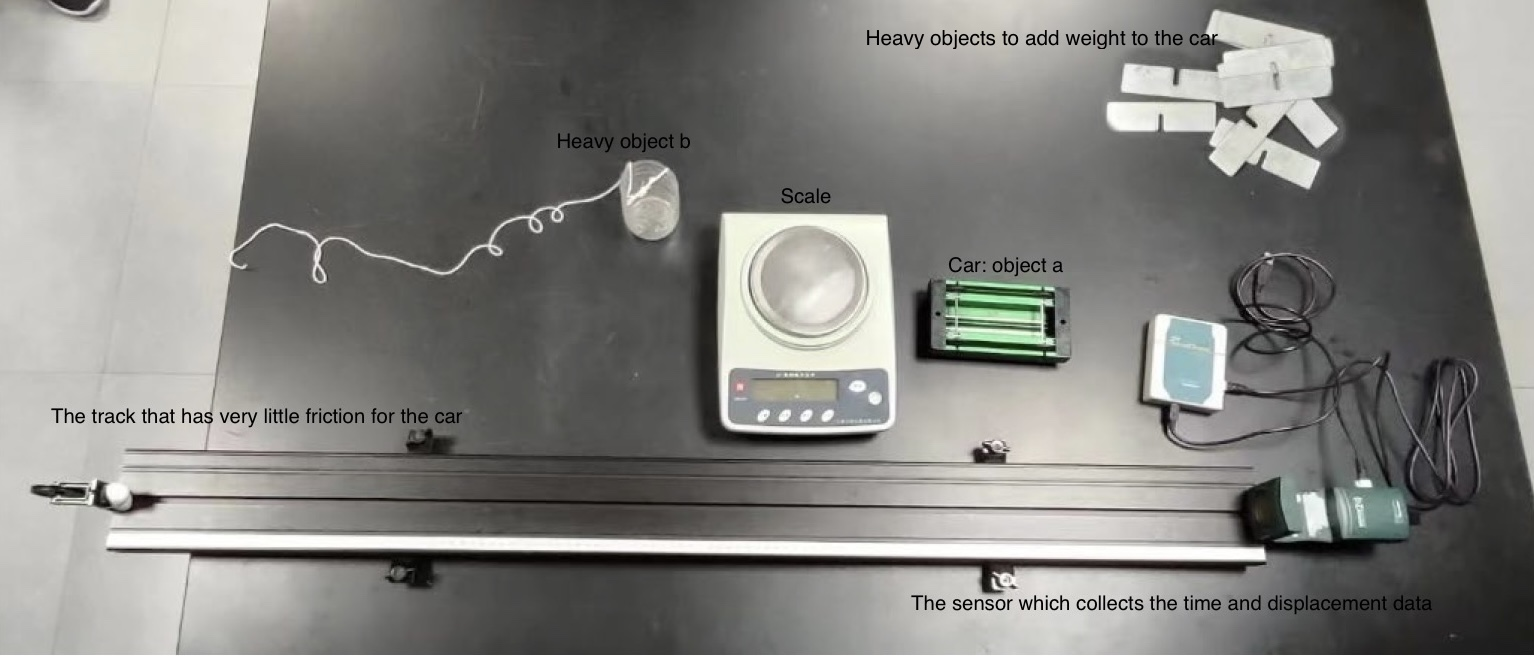
\includegraphics[width=.78\hsize]{setup01.jpeg}\\
  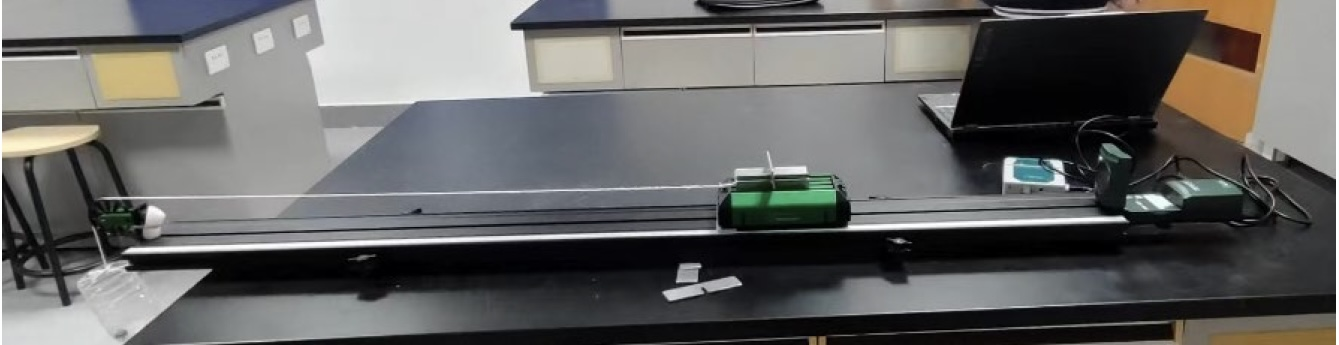
\includegraphics[width=.78\hsize]{setup02.jpeg}
  \caption{Set-up diagram for this experiment}
  \label{fig:setup}
\end{figure}

\subsection{Safety, Environmental or Ethical Concerns}

\begin{itemize}
  \item The car tied to a heavy object is very dangerous since it moves at a fast speed. To ensure safety, we surround the equipment with fences.
  \item The heavy objects added to the car is sharp and may cut people very easily. Thus we wear gloves when operating on these objects to prevent harm.
\end{itemize}

\section{Analysis}

\subsection{Raw Data Collection}

\begin{table}
  \centering
  \begin{tabular}{|c|c|c|c|}
    \hline
    \multirow{2}{*}{\vbox{\hbox{Total Mass $(m_a + m_b) / \text{g}$} \hbox{$\Delta (m_a + m_b) \pm 0.01 \text{g}$}}} & \multicolumn{3}{|c|}{\vbox{\hbox{Acceleration $a / m \cdot s^{-2}$} \hbox{$\Delta c = \pm 0.001 m \cdot s^{-2}$}}} \\
    \cline{2-4}
    & Trail 1 & Trail 2 & Trail 3 \\
    \hline
    $537.20$ & $0.432$ & $0.433$ & $0.430$ \\
    \hline
    $587.42$ & $0.365$ & $0.362$ & $0.370$ \\
    \hline
    $637.40$ & $0.321$ & $0.320$ & $0.316$ \\
    \hline
    $737.39$ & $0.255$ & $0.255$ & $0.256$ \\
    \hline
    $787.68$ & $0.233$ & $0.232$ & $0.227$ \\
    \hline
  \end{tabular}
  \caption{Raw data}
  \label{tab:raw}
\end{table}

We use the set of data given in table \ref{tab:raw} to give an example on how we processed each group of datum.

\subsection{Data Analysis}

Since we deduced before that acceleration is:
\[
  \frac{m_b \cdot g}{m_a + m_b}
\]
therefore we should first find the reciprocal of $m_a + m_b$ which is:
\[
  \frac{1}{537.20 \text{g}} = 1.86150 \times 10^{-3} \text{g}
\]
while its uncertainty is:
\[
  \Delta \left( \frac{1}{m_a + m_b} \right) = \left( \frac{0.01 \text{g}}{537.20 \text{g}} \right)^2 \cdot 1 = 3 \times 10^{-8} \text{g}^{-1}.
\]

Next we calculate the average of the velocity:
\[
  \bar{a} = \frac{a_1 + a_2 + a_3}{3} = \frac{0.432 + 0.433 + 0.430}{3} \text{m} / \text{s}^{-2} = 0.432 \text{m} / \text{s}^{-2}
\]
which uncertainty is:
\[
  \Delta \bar{a} = \frac{a_\text{max} - a_\text{min}}{2} = \frac{0.433 - 0.430}{2} \text{m} / \text{s}^{-2} = 0.002 \text{m} / \text{s}^{-2}.
\]

The table \ref{tab:psd} shows the processed data.

\begin{table}
  \Scentering
  \begin{tabular}{|c|c|c|c|}
    \hline
    \vbox{\hbox{Reciprocal of Total Mass} \hbox{$\frac{1}{m_a + m_b}/\text{kg}^{-1}$}} & \vbox{\hbox{Uncertainty of Reciprocal of Total Mass} \hbox{$\Delta \left( \frac{1}{m_a + m_b} \right)/\text{kg}^{-1}$}} & \vbox{\hbox{The Average of Acceleration} \hbox{$\bar{a}/\text{m} \cdot \text{s}^{-1}$}} & \vbox{\hbox{The Uncertainty of Acceleration} \hbox{$\Delta \bar{a}/\text{m} \cdot \text{s}^{-1}$}} \\
    \hline
    $1.8615 \times 10^{-3}$ & $3 \times 10^{-8}$ & $0.432$ & $0.002$ \\
    \hline
    $1.6976 \times 10^{-3}$ & $3 \times 10^{-8}$ & $0.366$ & $0.004$ \\
    \hline
    $1.5686 \times 10^{-3}$ & $3 \times 10^{-8}$ & $0.319$ & $0.003$ \\
    \hline
    $1.4544 \times 10^{-3}$ & $3 \times 10^{-8}$ & $0.281$ & $0.004$ \\
    \hline
    $1.3553 \times 10^{-3}$ & $3 \times 10^{-8}$ & $0.255$ & $0.001$ \\
    \hline
    $1.2697 \times 10^{-3}$ & $3 \times 10^{-8}$ & $0.231$ & $0.003$ \\
    \hline
  \end{tabular}
  \caption{Processed Data}
  \label{tab:psd}
\end{table}

\subsection{Processed Data Presentation}

\begin{figure}
  \centering
  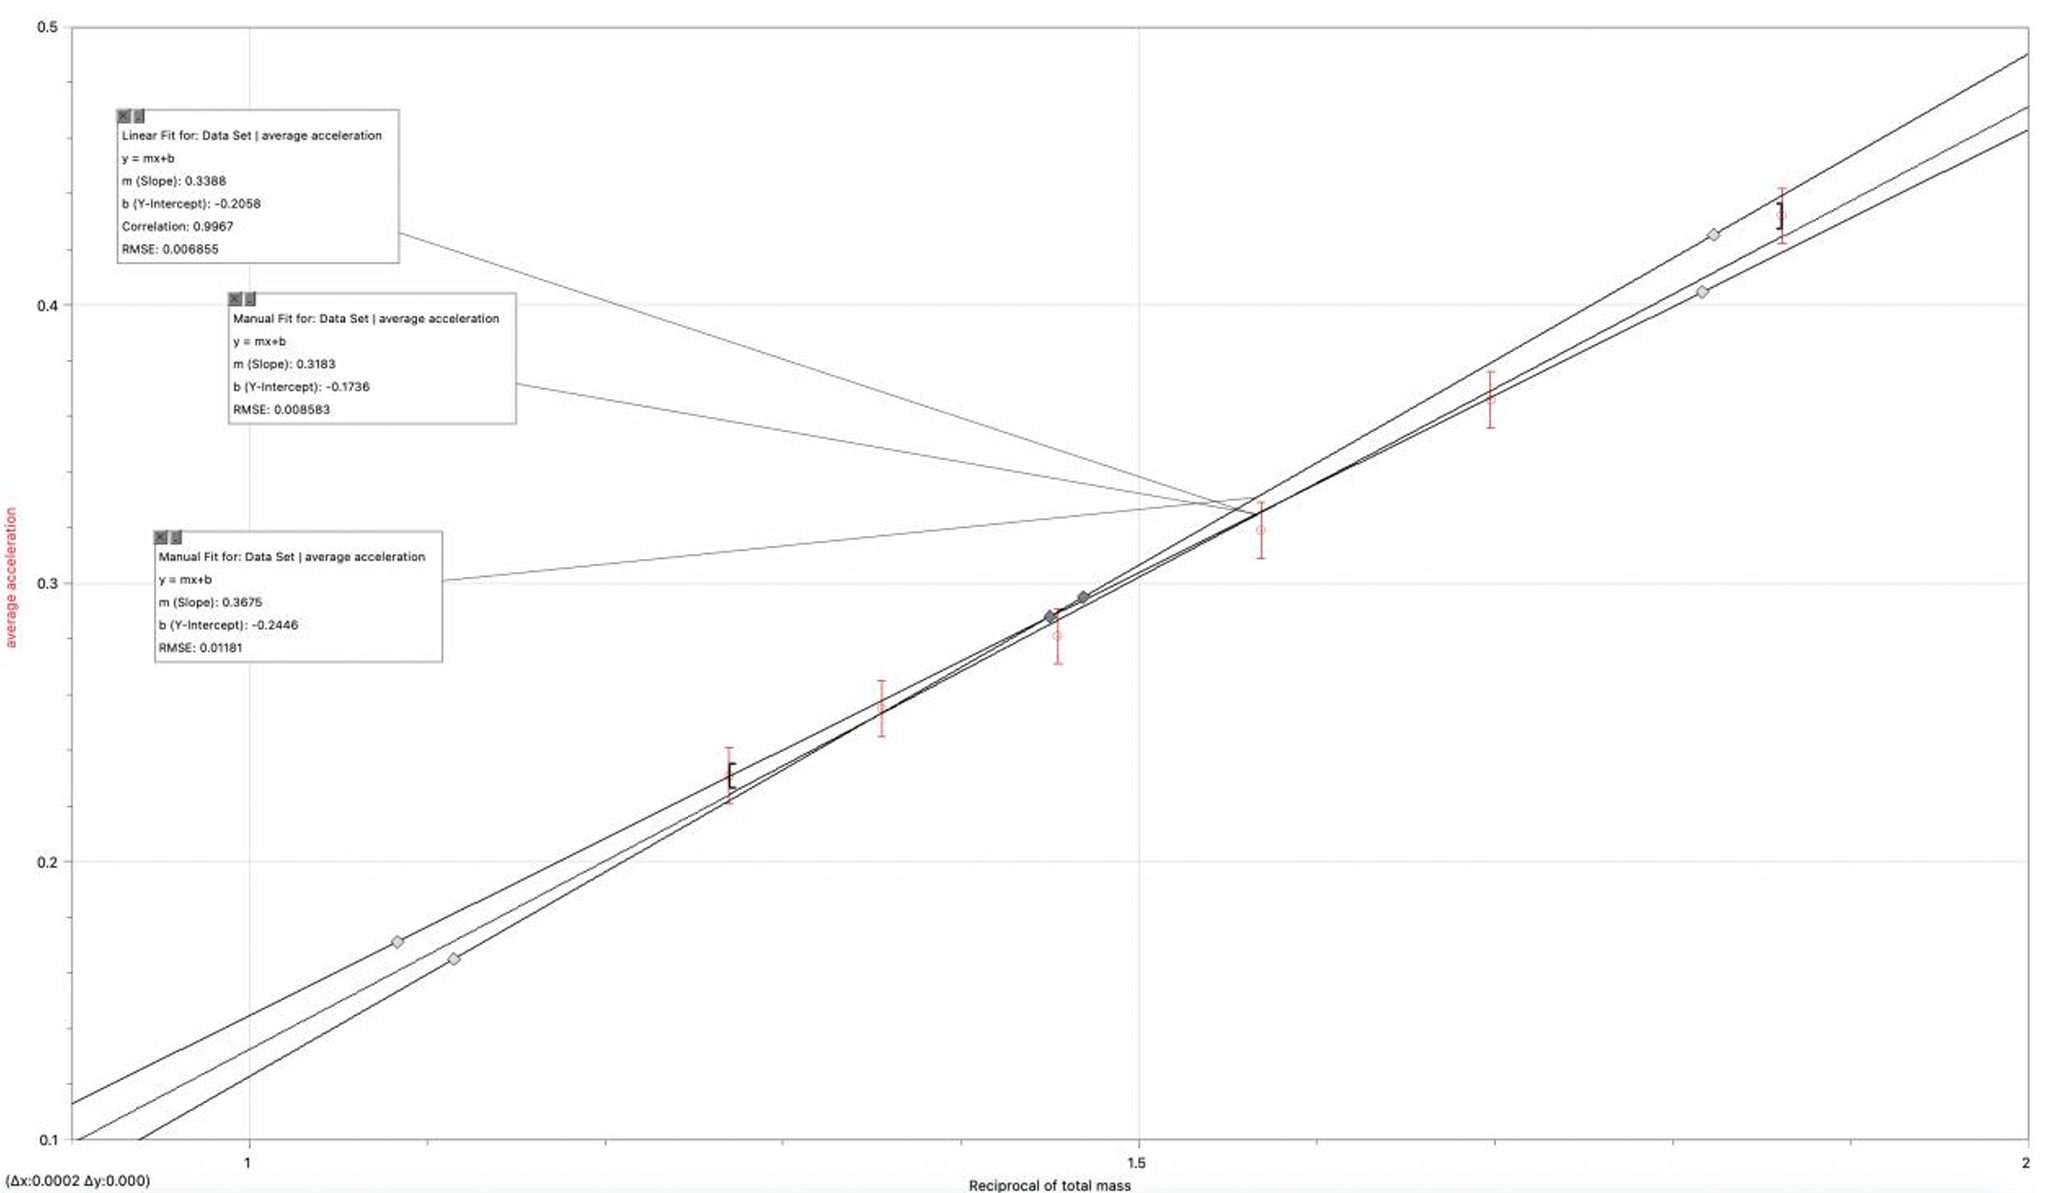
\includegraphics[width=.78\hsize]{psd.jpeg}
  \caption{Relationship between the average acceleration and the reciprocal of total mass}
  \label{fig:lpdt}
\end{figure}

The graph of the processeed data is shown in figure \ref{fig:lpdt}, and according to the deduction, we expect a proportional relationship while the graph shows that relationship
after we draw a best fit line that passes through all the points.
Also, the $\Delta \left( \frac{1}{m_a + m_b} \right)$ is smaller than the single measurement therefore can be negelected.

From this figure we can know that the gradient of best fit is $0.339$, while the maximum is $0.368$ and the minimum is $0.318$.
Its uncertainty calculated is:
\[
  \Delta k = \frac{k_\text{max} - k_\text{min}}{2} = 0.025 \approx 0.03.
\]
The relative uncertainty of $k$ is therefore $7.37\%$.

We can also know the $y$-intercept of the best fit line is $i_\text{best} = -0.206$.

Finally we can calculate the acceleration which is:
\[
  a = \frac{k}{m_a + m_b} + i_\text{best} = (0.339 \pm 0.025) \times \frac{1}{m_a + m_b} - 0.206.
\]

\end{document}
